\subsection{Thinking, Fast and Slow (Daniel Kahnemann)}

This book tells us the story of three pairs of (opposing) entities: That of System 1 and System 2, Econs and humans, and the experiencing and remembering selves.
System 1 and 2 are personalisations of two kinds of ways our brain approaches the world, through an intuitive understanding of the world and speedy decisions (system 1), and a slower, (more) rational system 2, which monitors system 1 and may take over when it doesn't 'agree' or is triggered. Econs are completely rational beings who should be left free to make their own choices, Humans are not and should be given help when making some decisions (tldr; read nudge for this part)
The experiencing self is the human that experiences each moment while the remembering self remembers that and is usually more powerful in making decisions
It is a book about behavioural economics though I found it to be more fitting to decision psychology, as it pertains to how we make decisions and think about them.
The main theme of the book is how we're not rational (though Kahnemann wants to make sure we don't interpret that as meaning we're irrational).
Personally I found many of the examples in the book to be quite insightful and they stimulated me towards reflecting on my own perspectiv on the matters, so I'll take a few to highlight what I mean;


\begin{itemize}[leftmargin=4cm]
\item[Heuristics] When we get a question that is harder to answer and would require quite some thinking our intuitive system (system 1) will usually answer a simpler question and propose its solution instead. Think for instance if you are asked whether you are happy with your life it should take quite a while to collect all the factors which can influence that, but we can also just fill in whether we are happy right now.
\item[The law of small numbers] Extreme cases are more likely to occur when you're looking at small numbers
\item[Pain] Would it be more painful an experience to add onto a torture with the same peak pain an additional 10 minutes of a bit lesser pain? No, it would actually reduce the amount of pain someone remembers (remembering selves have no concept of time)
\item[Asian Disease problem] The way we frame two treatments will have influence on which solution will be chosen which has a paradoxical effect.
\item[Storylines] If you add 10 slightly worse years to someone's life they'll think the entire life's worse than without those years, because the end matters so much.

\end{itemize}


\subsubsection{Concepts named}
As this book is meant to be about learning the concepts and being able to use them, I would be remiss if I did not list them all out to increase the ability of myself to recall them :)

\begin{itemize}[leftmargin=4cm]
\item[Anchoring Effect] When we compare things any numbers that are given are used as a relative setpoint. e.g. If we see a house on sale for 2 millions we'll go lower from there not get an entire different start bid like 2 tons. 
\item[Sunk Cost] Basically the gambler's fallacy, we shouldn't consider what we have already spent when making a choice, just the current state of things.
\item[Loss Aversion] All things considered, losses weigh more than gains both in the amount of emotion they cause and the amount of regret they spark. As such we tend to avoid sure losses and take gambles, while the opposite is the case for gains.
\item[Regression to mean] Luck/chance has a larger role in life than we'd usually like to imagine, which ends up to mean that if something goes well occasionally, that it will also go bad occasionally.
\item[Framing bias] Framing a question one way or another can influence how it is perceived (as a positive or negative outcome, good or bad solution)
\item[Availability bias] When asked how frequently something occurs, you'll think it occurs more frequently if it comes to mind more easily (think terrorist attacks)
\item[Cognitive load] We tend towards less cognitive load (stress on the brain). If something takes a lot of brain power, we'll want to avoid it more.
\item[The Confirmation bias] We tend to look for info that reinforces our own beliefs instead of adapting your beliefs to other facts which we tend to overlook.
\item[Correlation != Causation] No more need be said here
\item[Substitution] Answer a harder question with an easier one (sometimes without knowing)
\item[Causes $>>$ Facts] Humans don't want statistics, they want a sappy story.
\item[Halo effect] Kinda seeing things as black and white. Your first impression colours the story you draw of someone.
\item[Environmental bias] Your surroundings effect you more than you'd want to admit. A lot of posters of the great leader will tend to make you more loyal, sad to say.
\item[Less is more] If you add more detail to a situation you make it seem more likely while you actually reduce the probability (subsets!)

\end{itemize}

\paragraph{More info?}
Could always re-read the book, and I found that the following medium article was quite clear: \href{https://medium.com/swlh/every-chapter-of-thinking-fast-and-slow-in-7-minutes-5e6adf89cf39}{Every Chapter of Thinking Fast, and Slow in 7 Minutes}
\begin{figure}
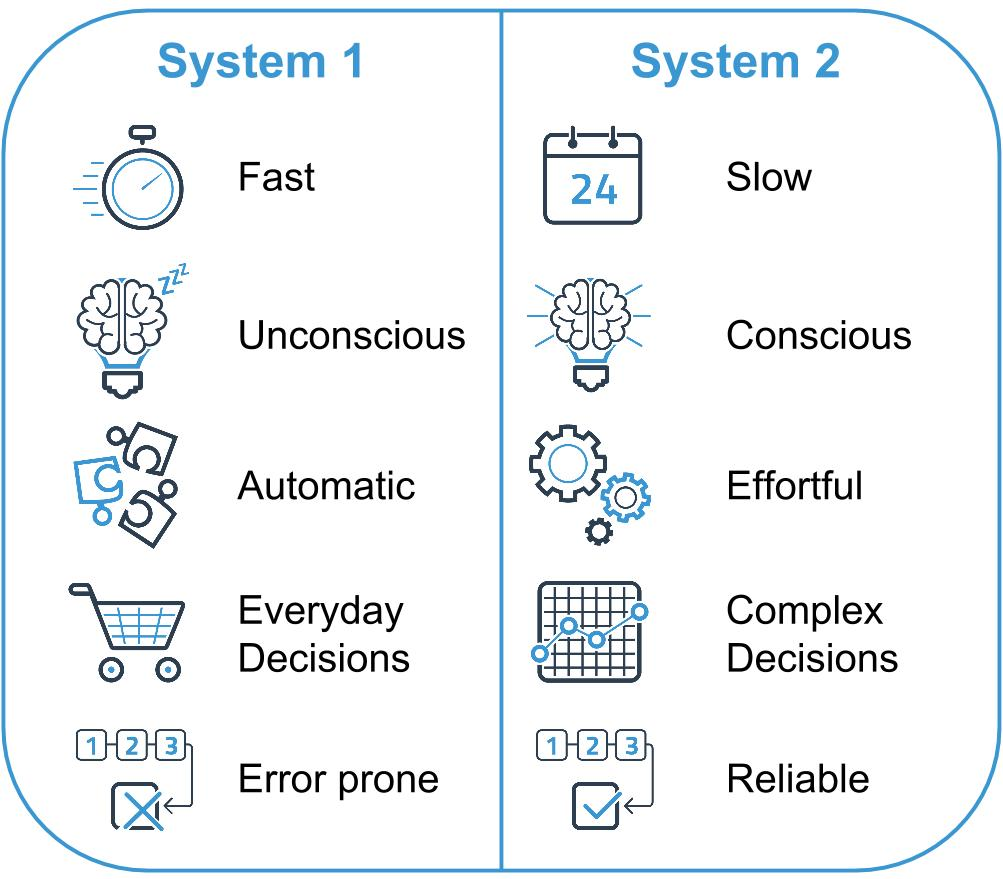
\includegraphics[scale=0.5]{summaries/thinking-fast-and-slow-systems.png}
\caption{The systems of the mind (useful overview)}
\end{figure}